\documentclass[11pt,a4paper]{article}

\usepackage[margin=1in]{geometry}
\usepackage{mathptmx}
\usepackage{amsmath}
\usepackage{amssymb}
\usepackage{amsthm}
\usepackage{braket}
\usepackage{tikz}
\usepackage{quantikz}
\usepackage{enumitem}
\usepackage{hyperref}
\usepackage{xcolor}

\definecolor{circuitblue}{RGB}{40,80,160}

\hypersetup{
    colorlinks=true,
    linkcolor=circuitblue,
    urlcolor=circuitblue,
    citecolor=circuitblue
}

\theoremstyle{definition}
\newtheorem{definition}{Definition}[section]
\newtheorem{example}{Example}[section]

\theoremstyle{remark}
\newtheorem*{intuition}{Intuition}
\newtheorem*{keypoint}{Key Point}

\pagestyle{plain}

\setlength{\parindent}{0pt}
\setlength{\parskip}{6pt}

\begin{document}

\begin{center}
    {\LARGE \textbf{Vector Spaces, Tensor Products, and Qubits}}\\[8pt]
    {\large QML}\\[12pt]
    \hrule
\end{center}

\vspace{12pt}
\tableofcontents
\newpage

%% ========================================================
\section{Why This Lecture Matters}
%% ========================================================

before u can do anything in quantum computing --- let alone quantum machine learning --- u need to be fluent in the math. and the math lives in vector spaces. specifically, complex vector spaces with inner products, bcs quantum mechanics is fundamentally abt amplitudes that r complex numbers.

this lecture builds up the entire mathematical foundation: vector spaces, inner products, dirac notation, tensor products, the bloch sphere, and density matrices. if u already know linear algebra, great --- but the quantum notation (bras, kets, brakets) takes some getting used to. and tensor products r where most people trip up when they first encounter multi-qubit systems.

\begin{keypoint}
everything in quantum computing is linear algebra over $\mathbb{C}$. if u understand vector spaces and tensor products, the rest of quantum computing is just applying these tools in clever ways.
\end{keypoint}

%% ========================================================
\section{Vector Spaces Over $\mathbb{C}$}
%% ========================================================

\subsection{Definition and Axioms}

\begin{definition}
a \textbf{vector space} $V$ over a field $\mathbb{F}$ (for us, $\mathbb{F} = \mathbb{C}$) is a set of objects called vectors, together with two operations:
\begin{enumerate}[label=(\roman*)]
    \item \textbf{vector addition}: $+: V \times V \to V$
    \item \textbf{scalar multiplication}: $\cdot: \mathbb{F} \times V \to V$
\end{enumerate}
satisfying the usual axioms: commutativity, associativity, existence of zero vector, existence of additive inverses, distributivity, and compatibility of scalar multiplication.
\end{definition}

for quantum computing, our vector space is $\mathbb{C}^n$ --- the space of $n$-dimensional column vectors with complex entries. for a single qubit, $n = 2$. for $k$ qubits, $n = 2^k$.

\begin{example}
the simplest quantum vector space is $\mathbb{C}^2$. a general element looks like:
\[
\mathbf{v} = \begin{pmatrix} \alpha \\ \beta \end{pmatrix}, \quad \alpha, \beta \in \mathbb{C}
\]
this is the state space of a single qubit. $\alpha$ and $\beta$ r called \textbf{probability amplitudes}.
\end{example}

\subsection{Linear Independence and Basis}

a set of vectors $\{v_1, v_2, \ldots, v_n\}$ is \textbf{linearly independent} if the only solution to
\[
c_1 v_1 + c_2 v_2 + \cdots + c_n v_n = 0
\]
is $c_1 = c_2 = \cdots = c_n = 0$.

\begin{definition}
a \textbf{basis} for $V$ is a linearly independent set that spans $V$. every vector in $V$ can be written as a unique linear combination of basis vectors. the number of basis vectors is the \textbf{dimension} of $V$.
\end{definition}

for $\mathbb{C}^2$, the standard basis is:
\[
e_0 = \begin{pmatrix} 1 \\ 0 \end{pmatrix}, \quad e_1 = \begin{pmatrix} 0 \\ 1 \end{pmatrix}
\]

in quantum computing, we call these the \textbf{computational basis states} and write them as $\ket{0}$ and $\ket{1}$ (more on this notation soon).

\subsection{Linear Maps and Matrices}

\begin{definition}
a \textbf{linear map} (or linear operator) $A: V \to W$ between vector spaces satisfies:
\begin{enumerate}[label=(\roman*)]
    \item $A(u + v) = A(u) + A(v)$
    \item $A(\alpha v) = \alpha A(v)$
\end{enumerate}
for all $u, v \in V$ and $\alpha \in \mathbb{C}$.
\end{definition}

once u pick a basis, every linear map can be represented as a matrix. in quantum computing, quantum gates r linear maps on the state space, so they r matrices. a gate on one qubit is a $2 \times 2$ matrix. a gate on two qubits is a $4 \times 4$ matrix. and so on.

\begin{keypoint}
quantum gates = matrices. quantum states = vectors. quantum computing = matrix-vector multiplication (plus measurement). thats the whole game at the mathematical level.
\end{keypoint}

\subsection{Special Classes of Matrices}

some matrix types come up constantly in quantum computing:

\textbf{Hermitian matrices:} $A = A^\dagger$ (equal to their own conjugate transpose). observables in quantum mechanics r hermitian. eigenvalues r always real.

\textbf{Unitary matrices:} $U U^\dagger = U^\dagger U = I$. quantum gates r unitary. they preserve inner products (and therefore probabilities).

\textbf{Normal matrices:} $A A^\dagger = A^\dagger A$. both hermitian and unitary matrices r normal. normal matrices have the spectral decomposition.

\begin{definition}
the \textbf{conjugate transpose} (or adjoint) of a matrix $A$ is denoted $A^\dagger$ and is obtained by transposing $A$ and taking the complex conjugate of every entry:
\[
(A^\dagger)_{ij} = \overline{A_{ji}}
\]
\end{definition}

\begin{example}
let $A = \begin{pmatrix} 1 & 2+i \\ 3i & 4 \end{pmatrix}$. then:
\[
A^\dagger = \begin{pmatrix} 1 & -3i \\ 2-i & 4 \end{pmatrix}
\]
\end{example}

%% ========================================================
\section{Inner Products and Norms}
%% ========================================================

\subsection{Inner Product Definition}

\begin{definition}
an \textbf{inner product} on a complex vector space $V$ is a function $\langle \cdot, \cdot \rangle: V \times V \to \mathbb{C}$ satisfying:
\begin{enumerate}[label=(\roman*)]
    \item \textbf{conjugate symmetry}: $\langle u, v \rangle = \overline{\langle v, u \rangle}$
    \item \textbf{linearity in second argument}: $\langle u, \alpha v + \beta w \rangle = \alpha \langle u, v \rangle + \beta \langle u, w \rangle$
    \item \textbf{positive definiteness}: $\langle v, v \rangle \geq 0$ with equality iff $v = 0$
\end{enumerate}
\end{definition}

note: physicists use the convention where the inner product is linear in the \textit{second} argument and conjugate-linear in the first. mathematicians often do it the other way. we follow the physics convention bcs thats wt quantum computing uses.

for $\mathbb{C}^n$, the standard inner product is:
\[
\boxed{\langle u, v \rangle = u^\dagger v = \sum_{i=1}^{n} \overline{u_i} v_i}
\]

\begin{example}
let $u = \begin{pmatrix} 1 \\ i \end{pmatrix}$ and $v = \begin{pmatrix} 2 \\ 3i \end{pmatrix}$. then:
\[
\langle u, v \rangle = u^\dagger v = \begin{pmatrix} 1 & -i \end{pmatrix} \begin{pmatrix} 2 \\ 3i \end{pmatrix} = 1 \cdot 2 + (-i)(3i) = 2 + 3 = 5
\]
\end{example}

\subsection{Norm and Distance}

the \textbf{norm} (length) of a vector is:
\[
\|v\| = \sqrt{\langle v, v \rangle}
\]

a vector with $\|v\| = 1$ is called a \textbf{unit vector} or \textbf{normalized vector}. quantum states r always normalized --- the total probability of all outcomes must equal 1.

\begin{keypoint}
if $\ket{\psi} = \alpha\ket{0} + \beta\ket{1}$, then the normalization condition is:
\[
\boxed{|\alpha|^2 + |\beta|^2 = 1}
\]
this is bcs $|\alpha|^2$ is the probability of measuring $\ket{0}$ and $|\beta|^2$ is the probability of measuring $\ket{1}$, and probabilities must sum to 1.
\end{keypoint}

\subsection{Orthogonality and Orthonormal Bases}

\begin{definition}
two vectors $u$ and $v$ r \textbf{orthogonal} if $\langle u, v \rangle = 0$. a basis $\{e_1, \ldots, e_n\}$ is \textbf{orthonormal} if:
\[
\langle e_i, e_j \rangle = \delta_{ij} = \begin{cases} 1 & \text{if } i = j \\ 0 & \text{if } i \neq j \end{cases}
\]
\end{definition}

the computational basis $\{\ket{0}, \ket{1}\}$ is orthonormal:
\[
\braket{0|0} = 1, \quad \braket{1|1} = 1, \quad \braket{0|1} = 0, \quad \braket{1|0} = 0
\]

\subsection{Gram-Schmidt Process}

given any basis, u can always turn it into an orthonormal basis using the gram-schmidt process. start with $\{v_1, v_2, \ldots\}$ and produce $\{e_1, e_2, \ldots\}$:

\begin{align}
e_1 &= \frac{v_1}{\|v_1\|} \\
e_2 &= \frac{v_2 - \langle e_1, v_2 \rangle e_1}{\|v_2 - \langle e_1, v_2 \rangle e_1\|}
\end{align}

and so on. subtract off the projections onto the already-found orthonormal vectors, then normalize.

\begin{example}
start with $v_1 = \begin{pmatrix} 1 \\ 1 \end{pmatrix}$ and $v_2 = \begin{pmatrix} 1 \\ -1 \end{pmatrix}$.

step 1: $e_1 = \frac{1}{\sqrt{2}} \begin{pmatrix} 1 \\ 1 \end{pmatrix}$

step 2: $\langle e_1, v_2 \rangle = \frac{1}{\sqrt{2}}(1 \cdot 1 + 1 \cdot (-1)) = 0$. so $v_2$ is already orthogonal to $e_1$. just normalize: $e_2 = \frac{1}{\sqrt{2}} \begin{pmatrix} 1 \\ -1 \end{pmatrix}$.

result: $\{e_1, e_2\}$ is an orthonormal basis. in quantum notation, this is $\{\ket{+}, \ket{-}\}$ --- the hadamard basis.
\end{example}

%% ========================================================
\section{Dirac Notation}
%% ========================================================

\subsection{Kets, Bras, and Brakets}

dirac notation is the standard language of quantum mechanics and quantum computing. its elegant and compact once u get used to it.

\begin{definition}
\textbf{ket}: a column vector $\ket{\psi} \in \mathbb{C}^n$. represents a quantum state.
\[
\ket{\psi} = \begin{pmatrix} \alpha_1 \\ \alpha_2 \\ \vdots \\ \alpha_n \end{pmatrix}
\]
\end{definition}

\begin{definition}
\textbf{bra}: the conjugate transpose of a ket. $\bra{\psi} = \ket{\psi}^\dagger$. its a row vector.
\[
\bra{\psi} = \begin{pmatrix} \overline{\alpha_1} & \overline{\alpha_2} & \cdots & \overline{\alpha_n} \end{pmatrix}
\]
\end{definition}

\begin{definition}
\textbf{braket}: the inner product of two states. $\braket{\phi|\psi} = \bra{\phi}\ket{\psi} \in \mathbb{C}$.
\end{definition}

\begin{keypoint}
the three key operations in dirac notation:
\begin{itemize}
    \item $\braket{\phi|\psi}$ --- inner product (a complex number)
    \item $\ket{\psi}\bra{\phi}$ --- outer product (a matrix)
    \item $A\ket{\psi}$ --- operator acting on a state (a new state)
\end{itemize}
\end{keypoint}

\subsection{The Computational Basis}

for a single qubit:
\[
\ket{0} = \begin{pmatrix} 1 \\ 0 \end{pmatrix}, \quad \ket{1} = \begin{pmatrix} 0 \\ 1 \end{pmatrix}
\]

any single qubit state can be written as:
\[
\boxed{\ket{\psi} = \alpha\ket{0} + \beta\ket{1}, \quad |\alpha|^2 + |\beta|^2 = 1}
\]

for $n$ qubits, the computational basis has $2^n$ elements:
\[
\ket{00\ldots0}, \ket{00\ldots1}, \ldots, \ket{11\ldots1}
\]

\begin{example}
a general two-qubit state:
\[
\ket{\psi} = \alpha_{00}\ket{00} + \alpha_{01}\ket{01} + \alpha_{10}\ket{10} + \alpha_{11}\ket{11}
\]
with $|\alpha_{00}|^2 + |\alpha_{01}|^2 + |\alpha_{10}|^2 + |\alpha_{11}|^2 = 1$.
\end{example}

\subsection{Outer Products and Projectors}

the outer product $\ket{\psi}\bra{\phi}$ is a matrix:
\[
\ket{0}\bra{0} = \begin{pmatrix} 1 \\ 0 \end{pmatrix} \begin{pmatrix} 1 & 0 \end{pmatrix} = \begin{pmatrix} 1 & 0 \\ 0 & 0 \end{pmatrix}
\]

\[
\ket{1}\bra{1} = \begin{pmatrix} 0 \\ 1 \end{pmatrix} \begin{pmatrix} 0 & 1 \end{pmatrix} = \begin{pmatrix} 0 & 0 \\ 0 & 1 \end{pmatrix}
\]

\begin{definition}
a \textbf{projector} onto a state $\ket{\psi}$ is $P = \ket{\psi}\bra{\psi}$. it satisfies $P^2 = P$ (idempotent) and $P^\dagger = P$ (hermitian).
\end{definition}

\begin{intuition}
projectors r the mathematical objects behind measurement. when u measure a qubit in the computational basis, ur effectively applying the projectors $\ket{0}\bra{0}$ and $\ket{1}\bra{1}$ to the state. the probability of getting outcome $j$ is $\bra{\psi}\ket{j}\bra{j}\ket{\psi} = |\braket{j|\psi}|^2$.
\end{intuition}

\subsection{Completeness Relation}

for any orthonormal basis $\{\ket{e_i}\}$:
\[
\boxed{\sum_i \ket{e_i}\bra{e_i} = I}
\]

this is called the \textbf{completeness relation} or \textbf{resolution of the identity}. its incredibly useful for inserting identities into expressions and changing bases.

\begin{example}
for the computational basis:
\[
\ket{0}\bra{0} + \ket{1}\bra{1} = \begin{pmatrix} 1 & 0 \\ 0 & 0 \end{pmatrix} + \begin{pmatrix} 0 & 0 \\ 0 & 1 \end{pmatrix} = \begin{pmatrix} 1 & 0 \\ 0 & 1 \end{pmatrix} = I
\]
\end{example}

\subsection{Spectral Decomposition}

\begin{definition}
every hermitian (or more generally, normal) operator $A$ can be written as:
\[
\boxed{A = \sum_i \lambda_i \ket{e_i}\bra{e_i}}
\]
where $\lambda_i$ r the eigenvalues and $\ket{e_i}$ r the corresponding orthonormal eigenvectors.
\end{definition}

this is huge in quantum computing. it tells u that every observable can be decomposed into projectors onto its eigenstates, weighted by eigenvalues. measurement outcomes r eigenvalues, and post-measurement states r eigenstates.

\begin{example}
the pauli Z matrix:
\[
Z = \begin{pmatrix} 1 & 0 \\ 0 & -1 \end{pmatrix} = (+1)\ket{0}\bra{0} + (-1)\ket{1}\bra{1}
\]
eigenvalues: $+1$ and $-1$. eigenstates: $\ket{0}$ and $\ket{1}$.
\end{example}

%% ========================================================
\section{Tensor Products}
%% ========================================================

\subsection{Why Tensor Products?}

when u have two separate quantum systems --- say qubit A and qubit B --- the combined system lives in the \textbf{tensor product} of their individual state spaces. this is one of the most important (and initially confusing) concepts in quantum computing.

if qubit A lives in $\mathbb{C}^2$ and qubit B lives in $\mathbb{C}^2$, the combined system lives in $\mathbb{C}^2 \otimes \mathbb{C}^2 = \mathbb{C}^4$.

\begin{keypoint}
$n$ qubits live in a $2^n$-dimensional hilbert space. this exponential growth of the state space is the source of quantum computing's potential power --- and also why simulating quantum systems classically is so hard.
\end{keypoint}

\subsection{Definition of the Tensor Product}

\begin{definition}
the \textbf{tensor product} of two vectors $\ket{u} \in \mathbb{C}^m$ and $\ket{v} \in \mathbb{C}^n$ is a vector $\ket{u} \otimes \ket{v} \in \mathbb{C}^{mn}$ defined by:
\[
\begin{pmatrix} u_1 \\ u_2 \\ \vdots \\ u_m \end{pmatrix} \otimes \begin{pmatrix} v_1 \\ v_2 \\ \vdots \\ v_n \end{pmatrix} = \begin{pmatrix} u_1 v_1 \\ u_1 v_2 \\ \vdots \\ u_1 v_n \\ u_2 v_1 \\ \vdots \\ u_m v_n \end{pmatrix}
\]
this is also called the \textbf{Kronecker product} when applied to matrices.
\end{definition}

we also write $\ket{u} \otimes \ket{v}$ as $\ket{u}\ket{v}$ or $\ket{uv}$ for short.

\begin{example}
the two-qubit computational basis states:
\begin{align}
\ket{00} &= \ket{0} \otimes \ket{0} = \begin{pmatrix} 1 \\ 0 \end{pmatrix} \otimes \begin{pmatrix} 1 \\ 0 \end{pmatrix} = \begin{pmatrix} 1 \\ 0 \\ 0 \\ 0 \end{pmatrix} \\[6pt]
\ket{01} &= \ket{0} \otimes \ket{1} = \begin{pmatrix} 1 \\ 0 \end{pmatrix} \otimes \begin{pmatrix} 0 \\ 1 \end{pmatrix} = \begin{pmatrix} 0 \\ 1 \\ 0 \\ 0 \end{pmatrix} \\[6pt]
\ket{10} &= \ket{1} \otimes \ket{0} = \begin{pmatrix} 0 \\ 1 \end{pmatrix} \otimes \begin{pmatrix} 1 \\ 0 \end{pmatrix} = \begin{pmatrix} 0 \\ 0 \\ 1 \\ 0 \end{pmatrix} \\[6pt]
\ket{11} &= \ket{1} \otimes \ket{1} = \begin{pmatrix} 0 \\ 1 \end{pmatrix} \otimes \begin{pmatrix} 0 \\ 1 \end{pmatrix} = \begin{pmatrix} 0 \\ 0 \\ 0 \\ 1 \end{pmatrix}
\end{align}
\end{example}

\subsection{Properties of the Tensor Product}

the tensor product is:
\begin{itemize}
    \item \textbf{bilinear}: $(\alpha\ket{u_1} + \beta\ket{u_2}) \otimes \ket{v} = \alpha(\ket{u_1} \otimes \ket{v}) + \beta(\ket{u_2} \otimes \ket{v})$
    \item \textbf{NOT commutative}: $\ket{u} \otimes \ket{v} \neq \ket{v} \otimes \ket{u}$ in general
    \item \textbf{associative}: $(\ket{u} \otimes \ket{v}) \otimes \ket{w} = \ket{u} \otimes (\ket{v} \otimes \ket{w})$
\end{itemize}

heres a visual picture of how tensor products build up multi-qubit spaces:

\begin{center}
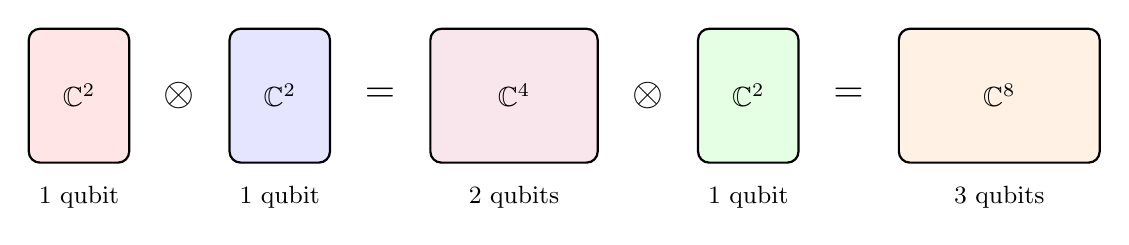
\begin{tikzpicture}[scale=0.85]
    % single qubit space
    \draw[thick, fill=red!10, rounded corners] (0,0) rectangle (1.5,2);
    \node at (0.75, 1) {$\mathbb{C}^2$};
    \node[below] at (0.75, -0.2) {\small 1 qubit};

    \node at (2.25, 1) {\Large $\otimes$};

    \draw[thick, fill=blue!10, rounded corners] (3,0) rectangle (4.5,2);
    \node at (3.75, 1) {$\mathbb{C}^2$};
    \node[below] at (3.75, -0.2) {\small 1 qubit};

    \node at (5.25, 1) {\Large $=$};

    \draw[thick, fill=purple!10, rounded corners] (6,0) rectangle (8.5,2);
    \node at (7.25, 1) {$\mathbb{C}^4$};
    \node[below] at (7.25, -0.2) {\small 2 qubits};

    \node at (9.25, 1) {\Large $\otimes$};

    \draw[thick, fill=green!10, rounded corners] (10,0) rectangle (11.5,2);
    \node at (10.75, 1) {$\mathbb{C}^2$};
    \node[below] at (10.75, -0.2) {\small 1 qubit};

    \node at (12.25, 1) {\Large $=$};

    \draw[thick, fill=orange!10, rounded corners] (13,0) rectangle (16,2);
    \node at (14.5, 1) {$\mathbb{C}^8$};
    \node[below] at (14.5, -0.2) {\small 3 qubits};
\end{tikzpicture}
\end{center}

each time u add a qubit, the dimension doubles: $2 \to 4 \to 8 \to 16 \to \ldots \to 2^n$. this exponential growth is wt makes quantum computing both powerful and hard to simulate classically.

\subsection{Tensor Products of Operators}

if $A$ acts on space $V$ and $B$ acts on space $W$, then $A \otimes B$ acts on $V \otimes W$:
\[
(A \otimes B)(\ket{u} \otimes \ket{v}) = (A\ket{u}) \otimes (B\ket{v})
\]

\begin{example}
applying X to the first qubit and I to the second qubit of $\ket{01}$:
\[
(X \otimes I)\ket{01} = (X\ket{0}) \otimes (I\ket{1}) = \ket{1} \otimes \ket{1} = \ket{11}
\]
\end{example}

the matrix form of $A \otimes B$ is the Kronecker product:
\[
A \otimes B = \begin{pmatrix} a_{11}B & a_{12}B & \cdots \\ a_{21}B & a_{22}B & \cdots \\ \vdots & & \ddots \end{pmatrix}
\]

\begin{example}
\[
X \otimes I = \begin{pmatrix} 0 & 1 \\ 1 & 0 \end{pmatrix} \otimes \begin{pmatrix} 1 & 0 \\ 0 & 1 \end{pmatrix} = \begin{pmatrix} 0 & 0 & 1 & 0 \\ 0 & 0 & 0 & 1 \\ 1 & 0 & 0 & 0 \\ 0 & 1 & 0 & 0 \end{pmatrix}
\]
\end{example}

\subsection{Product States vs Entangled States}

\begin{definition}
a state $\ket{\psi} \in V \otimes W$ is called a \textbf{product state} (or separable state) if it can be written as $\ket{\psi} = \ket{u} \otimes \ket{v}$ for some $\ket{u} \in V$, $\ket{v} \in W$. otherwise, its \textbf{entangled}.
\end{definition}

\begin{example}
$\ket{01} = \ket{0} \otimes \ket{1}$ is a product state.

the bell state $\ket{\Phi^+} = \frac{1}{\sqrt{2}}(\ket{00} + \ket{11})$ is entangled --- u \textbf{cannot} write it as $\ket{a} \otimes \ket{b}$ for any single-qubit states $\ket{a}$ and $\ket{b}$.
\end{example}

\begin{center}
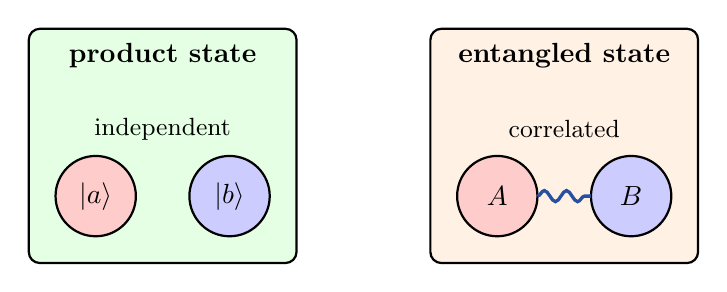
\begin{tikzpicture}[scale=0.85]
    % product state
    \draw[thick, rounded corners, fill=green!10] (-0.5, -0.5) rectangle (3.5, 3);
    \node[font=\bfseries] at (1.5, 2.6) {product state};
    \draw[thick, fill=red!20] (0.5, 0.5) circle (0.6);
    \node at (0.5, 0.5) {$\ket{a}$};
    \draw[thick, fill=blue!20] (2.5, 0.5) circle (0.6);
    \node at (2.5, 0.5) {$\ket{b}$};
    \node at (1.5, 1.5) {\small independent};

    % entangled state
    \draw[thick, rounded corners, fill=orange!10] (5.5, -0.5) rectangle (9.5, 3);
    \node[font=\bfseries] at (7.5, 2.6) {entangled state};
    \draw[thick, fill=red!20] (6.5, 0.5) circle (0.6);
    \node at (6.5, 0.5) {$A$};
    \draw[thick, fill=blue!20] (8.5, 0.5) circle (0.6);
    \node at (8.5, 0.5) {$B$};
    \draw[very thick, circuitblue, decorate, decoration={snake, amplitude=2pt, segment length=8pt}] (7.1, 0.5) -- (7.9, 0.5);
    \node at (7.5, 1.5) {\small correlated};
\end{tikzpicture}
\end{center}

\begin{intuition}
heres an easy way to check if a two-qubit state is entangled. write the state as a matrix:
\[
\ket{\psi} = \alpha_{00}\ket{00} + \alpha_{01}\ket{01} + \alpha_{10}\ket{10} + \alpha_{11}\ket{11} \quad \leftrightarrow \quad M = \begin{pmatrix} \alpha_{00} & \alpha_{01} \\ \alpha_{10} & \alpha_{11} \end{pmatrix}
\]
the state is a product state iff $\det(M) = 0$. if $\det(M) \neq 0$, its entangled.

for the bell state: $M = \frac{1}{\sqrt{2}}\begin{pmatrix} 1 & 0 \\ 0 & 1 \end{pmatrix}$, $\det(M) = \frac{1}{2} \neq 0$. entangled.
\end{intuition}

%% ========================================================
\section{Single Qubit States and the Bloch Sphere}
%% ========================================================

\subsection{The Qubit}

\begin{definition}
a \textbf{qubit} is a two-level quantum system. its state is a unit vector in $\mathbb{C}^2$:
\[
\ket{\psi} = \alpha\ket{0} + \beta\ket{1}, \quad |\alpha|^2 + |\beta|^2 = 1, \quad \alpha, \beta \in \mathbb{C}
\]
\end{definition}

since $\alpha$ and $\beta$ r complex numbers, a qubit has 4 real parameters. but the normalization constraint removes 1 degree of freedom, and the global phase is unobservable (more on this below), so a qubit has \textbf{2 real degrees of freedom}.

\subsection{Global Phase}

\begin{definition}
a \textbf{global phase} is a factor $e^{i\gamma}$ multiplying the entire state: $\ket{\psi'} = e^{i\gamma}\ket{\psi}$. global phases r physically unobservable bcs all measurement probabilities r unchanged:
\[
|\braket{j|e^{i\gamma}\psi}|^2 = |e^{i\gamma}|^2 |\braket{j|\psi}|^2 = |\braket{j|\psi}|^2
\]
\end{definition}

bcs of this, we can always choose $\alpha$ to be real and non-negative. this gives us the standard parameterization.

\subsection{The Bloch Sphere}

using the freedom to remove the global phase, any single qubit state can be written as:
\[
\boxed{\ket{\psi} = \cos\frac{\theta}{2}\ket{0} + e^{i\phi}\sin\frac{\theta}{2}\ket{1}}
\]
where $0 \leq \theta \leq \pi$ and $0 \leq \phi < 2\pi$.

this parameterization maps every qubit state to a point on the unit sphere in $\mathbb{R}^3$ called the \textbf{Bloch sphere}.

\begin{center}
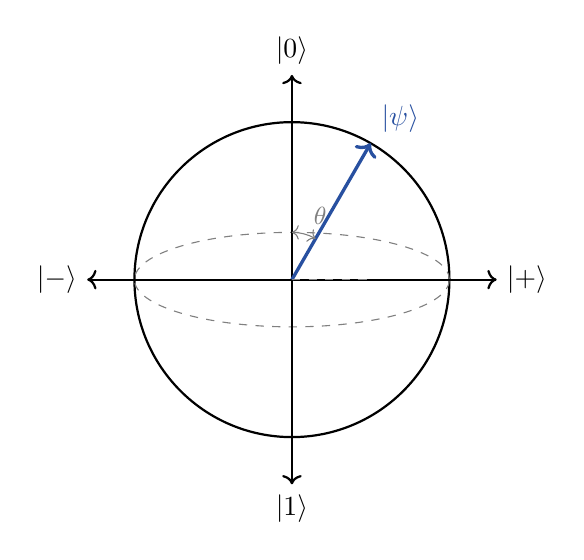
\begin{tikzpicture}[scale=2]
    % sphere
    \draw[thick] (0,0) circle (1);
    \draw[dashed, gray] (0,0) ellipse (1 and 0.3);

    % axes
    \draw[->, thick] (0,0) -- (0,1.3) node[above] {$\ket{0}$};
    \draw[->, thick] (0,0) -- (0,-1.3) node[below] {$\ket{1}$};
    \draw[->, thick] (0,0) -- (1.3,0) node[right] {$\ket{+}$};
    \draw[->, thick] (0,0) -- (-1.3,0) node[left] {$\ket{-}$};

    % state vector
    \draw[->, very thick, circuitblue] (0,0) -- (0.5,0.866) node[above right] {$\ket{\psi}$};

    % angles
    \draw[dashed, gray] (0,0) -- (0.5,0);
    \draw[<->, gray] (0,0.3) arc (90:60:0.3) node[midway, above right, font=\small] {$\theta$};
\end{tikzpicture}
\end{center}

\begin{keypoint}
key states on the bloch sphere:
\begin{itemize}
    \item north pole ($\theta = 0$): $\ket{0}$
    \item south pole ($\theta = \pi$): $\ket{1}$
    \item equator ($\theta = \pi/2$): equal superposition states
    \item $\ket{+} = \frac{1}{\sqrt{2}}(\ket{0} + \ket{1})$: positive x-axis
    \item $\ket{-} = \frac{1}{\sqrt{2}}(\ket{0} - \ket{1})$: negative x-axis
    \item $\ket{+i} = \frac{1}{\sqrt{2}}(\ket{0} + i\ket{1})$: positive y-axis
    \item $\ket{-i} = \frac{1}{\sqrt{2}}(\ket{0} - i\ket{1})$: negative y-axis
\end{itemize}
\end{keypoint}

\begin{intuition}
the bloch sphere is only for single qubits. for multi-qubit systems, the state space is much more complex and cant be visualized as a simple sphere. this is one reason why quantum computing is hard to think abt --- ur intuition from the bloch sphere doesnt directly extend to multiple qubits.

also note: orthogonal quantum states r \textbf{antipodal} on the bloch sphere (opposite sides). $\ket{0}$ and $\ket{1}$ r orthogonal and sit at the north and south poles. $\ket{+}$ and $\ket{-}$ r orthogonal and sit on opposite ends of the x-axis.
\end{intuition}

\subsection{Rotations on the Bloch Sphere}

single qubit gates correspond to rotations on the bloch sphere. the pauli matrices generate rotations around the x, y, and z axes:

\begin{align}
R_x(\theta) &= e^{-i\theta X/2} = \cos\frac{\theta}{2}I - i\sin\frac{\theta}{2}X = \begin{pmatrix} \cos\frac{\theta}{2} & -i\sin\frac{\theta}{2} \\ -i\sin\frac{\theta}{2} & \cos\frac{\theta}{2} \end{pmatrix} \\[8pt]
R_y(\theta) &= e^{-i\theta Y/2} = \cos\frac{\theta}{2}I - i\sin\frac{\theta}{2}Y = \begin{pmatrix} \cos\frac{\theta}{2} & -\sin\frac{\theta}{2} \\ \sin\frac{\theta}{2} & \cos\frac{\theta}{2} \end{pmatrix} \\[8pt]
R_z(\theta) &= e^{-i\theta Z/2} = \cos\frac{\theta}{2}I - i\sin\frac{\theta}{2}Z = \begin{pmatrix} e^{-i\theta/2} & 0 \\ 0 & e^{i\theta/2} \end{pmatrix}
\end{align}

any single qubit unitary can be decomposed as:
\[
\boxed{U = e^{i\alpha} R_z(\beta) R_y(\gamma) R_z(\delta)}
\]
for some angles $\alpha, \beta, \gamma, \delta$. this is the ZYZ decomposition and its important for quantum compilation.

%% ========================================================
\section{Computational Basis, Superposition, and Measurement}
%% ========================================================

\subsection{Superposition}

the ability of a qubit to be in a linear combination of $\ket{0}$ and $\ket{1}$ is called \textbf{superposition}. this is NOT the same as saying the qubit is ``both 0 and 1 at the same time'' --- thats a pop-science misunderstanding.

\begin{keypoint}
superposition means the qubit's state is described by a vector with nonzero components in multiple basis directions. when u measure, u get a definite outcome, and the probabilities r determined by the amplitudes. the qubit is not ``both'' --- its in a state that has no classical analogue.
\end{keypoint}

\subsection{Measurement in the Computational Basis}

\begin{definition}
\textbf{measurement} in the computational basis of a state $\ket{\psi} = \alpha\ket{0} + \beta\ket{1}$:
\begin{itemize}
    \item outcome $0$ with probability $|\alpha|^2$, post-measurement state $\ket{0}$
    \item outcome $1$ with probability $|\beta|^2$, post-measurement state $\ket{1}$
\end{itemize}
measurement is \textbf{irreversible} --- it destroys the superposition.
\end{definition}

for a multi-qubit state $\ket{\psi} = \sum_x \alpha_x \ket{x}$, measuring all qubits gives outcome $x$ with probability $|\alpha_x|^2$.

\begin{example}
measure $\ket{\psi} = \frac{1}{\sqrt{3}}\ket{0} + \sqrt{\frac{2}{3}}\ket{1}$:
\begin{itemize}
    \item $P(\text{outcome } 0) = |1/\sqrt{3}|^2 = 1/3$
    \item $P(\text{outcome } 1) = |\sqrt{2/3}|^2 = 2/3$
\end{itemize}
\end{example}

\subsection{Measurement in Other Bases}

u can measure in any orthonormal basis, not just the computational basis. measuring in the basis $\{\ket{b_0}, \ket{b_1}\}$ gives:
\begin{itemize}
    \item outcome $b_0$ with probability $|\braket{b_0|\psi}|^2$
    \item outcome $b_1$ with probability $|\braket{b_1|\psi}|^2$
\end{itemize}

\begin{example}
measure $\ket{0}$ in the $\{\ket{+}, \ket{-}\}$ basis:
\begin{itemize}
    \item $P(+) = |\braket{+|0}|^2 = |1/\sqrt{2}|^2 = 1/2$
    \item $P(-) = |\braket{-|0}|^2 = |1/\sqrt{2}|^2 = 1/2$
\end{itemize}
makes sense --- $\ket{0}$ is an equal superposition of $\ket{+}$ and $\ket{-}$, so measuring in the hadamard basis gives 50/50.
\end{example}

\subsection{Partial Measurement}

for multi-qubit systems, u can measure just some of the qubits. this is called \textbf{partial measurement} and its crucial for quantum algorithms.

\begin{example}
consider $\ket{\psi} = \frac{1}{\sqrt{2}}\ket{00} + \frac{1}{2}\ket{01} + \frac{1}{2}\ket{11}$.

measure only the first qubit:
\begin{itemize}
    \item $P(\text{first qubit} = 0) = |1/\sqrt{2}|^2 + |1/2|^2 = 1/2 + 1/4 = 3/4$

    post-measurement state: $\frac{1/\sqrt{2}\ket{00} + 1/2\ket{01}}{\sqrt{3/4}} = \frac{2}{\sqrt{6}}\ket{00} + \frac{1}{\sqrt{6}}\ket{01} = \ket{0}\left(\frac{2}{\sqrt{6}}\ket{0} + \frac{1}{\sqrt{6}}\ket{1}\right)$

    \item $P(\text{first qubit} = 1) = |1/2|^2 = 1/4$

    post-measurement state: $\ket{11}$
\end{itemize}
\end{example}

\subsection{Born Rule and Measurement Postulate}

the \textbf{Born rule} is the fundamental connection between the mathematical formalism and experimental outcomes:

\[
\boxed{P(\text{outcome } i) = \bra{\psi}M_i^\dagger M_i\ket{\psi}}
\]

for projective measurements, $M_i = \ket{i}\bra{i}$ and this simplifies to $P(i) = |\braket{i|\psi}|^2$.

the most general measurement is described by a set of operators $\{M_i\}$ satisfying the \textbf{completeness relation}:
\[
\sum_i M_i^\dagger M_i = I
\]

%% ========================================================
\section{Density Matrices}
%% ========================================================

\subsection{Why Density Matrices?}

so far weve been describing quantum states as kets (state vectors). this works fine for \textbf{pure states} --- states we have complete knowledge of. but in practice, quantum systems r often in \textbf{mixed states} --- statistical mixtures of pure states. this happens bcs of:

\begin{itemize}
    \item noise and decoherence
    \item partial measurements (tracing out part of a system)
    \item classical uncertainty about which state was prepared
\end{itemize}

density matrices r the general framework that handles both pure and mixed states.

\subsection{Definition}

\begin{definition}
the \textbf{density matrix} (or density operator) of a quantum system is:
\[
\boxed{\rho = \sum_i p_i \ket{\psi_i}\bra{\psi_i}}
\]
where $p_i \geq 0$, $\sum_i p_i = 1$, and $\ket{\psi_i}$ r (not necessarily orthogonal) pure states. the system is in state $\ket{\psi_i}$ with classical probability $p_i$.
\end{definition}

properties of density matrices:
\begin{enumerate}[label=(\roman*)]
    \item $\rho$ is hermitian: $\rho = \rho^\dagger$
    \item $\rho$ is positive semidefinite: $\bra{v}\rho\ket{v} \geq 0$ for all $\ket{v}$
    \item $\text{tr}(\rho) = 1$ (trace equals 1)
\end{enumerate}

\begin{keypoint}
how to tell pure from mixed:
\begin{itemize}
    \item \textbf{pure state}: $\rho = \ket{\psi}\bra{\psi}$, $\text{tr}(\rho^2) = 1$, $\rho^2 = \rho$
    \item \textbf{mixed state}: $\rho = \sum_i p_i \ket{\psi_i}\bra{\psi_i}$ with at least two terms, $\text{tr}(\rho^2) < 1$
\end{itemize}
$\text{tr}(\rho^2)$ is called the \textbf{purity} of the state.
\end{keypoint}

\subsection{Examples}

\begin{example}
the density matrix of the pure state $\ket{+} = \frac{1}{\sqrt{2}}(\ket{0} + \ket{1})$:
\[
\rho = \ket{+}\bra{+} = \frac{1}{2}\begin{pmatrix} 1 & 1 \\ 1 & 1 \end{pmatrix}
\]
purity: $\text{tr}(\rho^2) = \text{tr}\left(\frac{1}{4}\begin{pmatrix} 2 & 2 \\ 2 & 2 \end{pmatrix}\right) = \frac{1}{4}(2+2) = 1$. pure state confirmed.
\end{example}

\begin{example}
the maximally mixed state (no information at all):
\[
\rho = \frac{1}{2}\ket{0}\bra{0} + \frac{1}{2}\ket{1}\bra{1} = \frac{1}{2}\begin{pmatrix} 1 & 0 \\ 0 & 1 \end{pmatrix} = \frac{I}{2}
\]
purity: $\text{tr}(\rho^2) = \text{tr}(I/4) = 1/2 < 1$. maximally mixed.
\end{example}

\subsection{Measurement with Density Matrices}

the probability of outcome $i$ when measuring state $\rho$:
\[
P(i) = \text{tr}(M_i^\dagger M_i \rho)
\]

for projective measurement in the computational basis:
\[
P(j) = \text{tr}(\ket{j}\bra{j}\rho) = \bra{j}\rho\ket{j} = \rho_{jj}
\]

so the diagonal elements of the density matrix in the computational basis directly give u the measurement probabilities. the off-diagonal elements (called \textbf{coherences}) encode information abt superposition.

\subsection{Time Evolution}

for a pure state: $\ket{\psi} \to U\ket{\psi}$.

for a density matrix:
\[
\boxed{\rho \to U\rho U^\dagger}
\]

this is the density matrix version of applying a quantum gate.

\subsection{Partial Trace and Reduced Density Matrices}

\begin{definition}
the \textbf{partial trace} over subsystem B of a bipartite state $\rho_{AB}$ gives the reduced density matrix of subsystem A:
\[
\rho_A = \text{tr}_B(\rho_{AB}) = \sum_j (I_A \otimes \bra{j}_B) \rho_{AB} (I_A \otimes \ket{j}_B)
\]
where $\{\ket{j}_B\}$ is any orthonormal basis for B.
\end{definition}

\begin{example}
consider the bell state $\ket{\Phi^+} = \frac{1}{\sqrt{2}}(\ket{00} + \ket{11})$. the density matrix is:
\[
\rho_{AB} = \ket{\Phi^+}\bra{\Phi^+} = \frac{1}{2}(\ket{00}\bra{00} + \ket{00}\bra{11} + \ket{11}\bra{00} + \ket{11}\bra{11})
\]

tracing out qubit B:
\[
\rho_A = \text{tr}_B(\rho_{AB}) = \frac{1}{2}(\ket{0}\bra{0} + \ket{1}\bra{1}) = \frac{I}{2}
\]

the reduced state of qubit A is maximally mixed, even tho the global state is pure. this is the signature of entanglement.
\end{example}

\begin{intuition}
the partial trace is wt happens when u ``forget'' or ``ignore'' part of a quantum system. if two qubits r entangled and u only look at one of them, that qubit appears to be in a mixed state. the information is in the correlations between the qubits, not in either qubit individually. this is fundamentally diff from classical correlations.
\end{intuition}

%% ========================================================
\section{Important Bases and Common States}
%% ========================================================

\subsection{The Three Standard Bases}

these r the three most common single-qubit bases. they correspond to measurement along the x, y, and z axes of the bloch sphere:

\textbf{Z-basis} (computational basis):
\[
\ket{0} = \begin{pmatrix} 1 \\ 0 \end{pmatrix}, \quad \ket{1} = \begin{pmatrix} 0 \\ 1 \end{pmatrix}
\]

\textbf{X-basis} (hadamard basis):
\[
\ket{+} = \frac{1}{\sqrt{2}}(\ket{0} + \ket{1}), \quad \ket{-} = \frac{1}{\sqrt{2}}(\ket{0} - \ket{1})
\]

\textbf{Y-basis}:
\[
\ket{+i} = \frac{1}{\sqrt{2}}(\ket{0} + i\ket{1}), \quad \ket{-i} = \frac{1}{\sqrt{2}}(\ket{0} - i\ket{1})
\]

\subsection{Bell States}

the four bell states form an orthonormal basis for the two-qubit system. they r maximally entangled:

\begin{align}
\ket{\Phi^+} &= \frac{1}{\sqrt{2}}(\ket{00} + \ket{11}) \\
\ket{\Phi^-} &= \frac{1}{\sqrt{2}}(\ket{00} - \ket{11}) \\
\ket{\Psi^+} &= \frac{1}{\sqrt{2}}(\ket{01} + \ket{10}) \\
\ket{\Psi^-} &= \frac{1}{\sqrt{2}}(\ket{01} - \ket{10})
\end{align}

\begin{keypoint}
the bell states r the building blocks of quantum information. they show up everywhere --- teleportation, superdense coding, entanglement swapping, quantum key distribution. u can create them with just a hadamard gate and a CNOT.
\end{keypoint}

heres how to prepare each bell state using circuits:

\textbf{preparing $\ket{\Phi^+}$:}
\begin{center}
\begin{quantikz}
\lstick{$\ket{0}$} & \gate{H} & \ctrl{1} & \qw & \rstick{$\frac{1}{\sqrt{2}}(\ket{00}+\ket{11})$} \\
\lstick{$\ket{0}$} & \qw & \targ{} & \qw &
\end{quantikz}
\end{center}

step by step: $\ket{00} \xrightarrow{H \otimes I} \frac{1}{\sqrt{2}}(\ket{0}+\ket{1})\ket{0} = \frac{1}{\sqrt{2}}(\ket{00}+\ket{10}) \xrightarrow{\text{CNOT}} \frac{1}{\sqrt{2}}(\ket{00}+\ket{11})$.

\textbf{preparing all four bell states:}
\begin{center}
\begin{quantikz}
\lstick{$\ket{b_1}$} & \gate{X}  & \gate{H} & \ctrl{1} & \qw \\
\lstick{$\ket{b_0}$} & \gate{X}  & \qw & \targ{} & \qw
\end{quantikz}
\end{center}
where $b_1 b_0 = 00 \to \ket{\Phi^+}$, $01 \to \ket{\Psi^+}$, $10 \to \ket{\Phi^-}$, $11 \to \ket{\Psi^-}$. (the $X$ gates r only applied when the corresponding input bit is 1.)

\subsection{GHZ and W States}

for three or more qubits, there r multiple inequivalent types of entanglement:

\textbf{GHZ state} (Greenberger-Horne-Zeilinger):
\[
\ket{GHZ} = \frac{1}{\sqrt{2}}(\ket{000} + \ket{111})
\]

\textbf{W state}:
\[
\ket{W} = \frac{1}{\sqrt{3}}(\ket{001} + \ket{010} + \ket{100})
\]

\begin{intuition}
GHZ and W states r fundamentally diff types of entanglement. if u lose one qubit of a GHZ state (trace it out), the remaining two qubits r in a separable mixed state --- all the entanglement is destroyed. but if u lose one qubit of a W state, the remaining two qubits r still entangled. W state entanglement is more ``robust'' in this sense.
\end{intuition}

\textbf{GHZ preparation circuit:}
\begin{center}
\begin{quantikz}
\lstick{$\ket{0}$} & \gate{H} & \ctrl{1} & \qw & \qw & \rstick{$\ket{GHZ}$} \\
\lstick{$\ket{0}$} & \qw & \targ{} & \ctrl{1} & \qw & \\
\lstick{$\ket{0}$} & \qw & \qw & \targ{} & \qw &
\end{quantikz}
\end{center}

pattern: hadamard on the first qubit, then cascade CNOTs downward. for $n$ qubits: 1 $H$ gate + $(n-1)$ CNOTs. the resulting state is $\frac{1}{\sqrt{2}}(\ket{00\ldots0} + \ket{11\ldots1})$.

%% --- measurement in different bases ---

\textbf{measurement in different bases:}

to measure in the Z-basis, just measure directly. to measure in other bases, apply a basis-change gate first:

\begin{center}
\begin{quantikz}
\lstick{$\ket{\psi}$} & \qw & \meter{Z} && \lstick{$\ket{\psi}$} & \gate{H} & \meter{X} && \lstick{$\ket{\psi}$} & \gate{S^\dagger} & \gate{H} & \meter{Y}
\end{quantikz}
\end{center}

measuring in the X-basis = apply $H$ then measure in Z. measuring in the Y-basis = apply $S^\dagger H$ then measure in Z. this is bcs $H\ket{+} = \ket{0}$ and $H\ket{-} = \ket{1}$, so the hadamard rotates the X-basis onto the Z-basis.

%% ========================================================
\section{Worked Examples and Exercises}
%% ========================================================

\subsection{Example: Inner Product Calculations}

\begin{example}
compute $\braket{+|-}$:
\begin{align}
\braket{+|-} &= \left(\frac{1}{\sqrt{2}}(\bra{0} + \bra{1})\right)\left(\frac{1}{\sqrt{2}}(\ket{0} - \ket{1})\right) \\
&= \frac{1}{2}(\braket{0|0} - \braket{0|1} + \braket{1|0} - \braket{1|1}) \\
&= \frac{1}{2}(1 - 0 + 0 - 1) = 0
\end{align}
$\ket{+}$ and $\ket{-}$ r orthogonal, as expected.
\end{example}

\begin{example}
compute $\braket{0|+}$:
\[
\braket{0|+} = \bra{0}\left(\frac{1}{\sqrt{2}}(\ket{0} + \ket{1})\right) = \frac{1}{\sqrt{2}}(\braket{0|0} + \braket{0|1}) = \frac{1}{\sqrt{2}}
\]
so the probability of measuring $\ket{+}$ in state $\ket{0}$ and getting 0 is $|\braket{0|+}|^2 = 1/2$.
\end{example}

\subsection{Example: Tensor Product Calculations}

\begin{example}
verify that $\ket{+} \otimes \ket{0}$ is a product state by writing it explicitly:
\begin{align}
\ket{+} \otimes \ket{0} &= \frac{1}{\sqrt{2}}(\ket{0} + \ket{1}) \otimes \ket{0} \\
&= \frac{1}{\sqrt{2}}(\ket{0} \otimes \ket{0} + \ket{1} \otimes \ket{0}) \\
&= \frac{1}{\sqrt{2}}(\ket{00} + \ket{10}) \\
&= \frac{1}{\sqrt{2}}\begin{pmatrix} 1 \\ 0 \\ 1 \\ 0 \end{pmatrix}
\end{align}
\end{example}

\begin{example}
show that $\ket{\Psi^-} = \frac{1}{\sqrt{2}}(\ket{01} - \ket{10})$ is entangled.

write the coefficient matrix: $M = \frac{1}{\sqrt{2}}\begin{pmatrix} 0 & 1 \\ -1 & 0 \end{pmatrix}$.

$\det(M) = \frac{1}{2}(0 \cdot 0 - 1 \cdot (-1)) = \frac{1}{2} \neq 0$.

since $\det(M) \neq 0$, the state is entangled.
\end{example}

\subsection{Example: Density Matrix Calculations}

\begin{example}
compute the density matrix and purity of the state $\ket{\psi} = \frac{1}{\sqrt{3}}\ket{0} + \sqrt{\frac{2}{3}}\ket{1}$.

\[
\rho = \ket{\psi}\bra{\psi} = \begin{pmatrix} 1/3 & \sqrt{2}/3 \\ \sqrt{2}/3 & 2/3 \end{pmatrix}
\]

\[
\rho^2 = \begin{pmatrix} 1/3 & \sqrt{2}/3 \\ \sqrt{2}/3 & 2/3 \end{pmatrix}^2 = \begin{pmatrix} 1/9 + 2/9 & \sqrt{2}/9 + 2\sqrt{2}/9 \\ \sqrt{2}/9 + 2\sqrt{2}/9 & 2/9 + 4/9 \end{pmatrix} = \begin{pmatrix} 1/3 & \sqrt{2}/3 \\ \sqrt{2}/3 & 2/3 \end{pmatrix}
\]

$\text{tr}(\rho^2) = 1/3 + 2/3 = 1$. pure state, as expected.
\end{example}

\begin{example}
consider a classical coin flip that prepares $\ket{0}$ with probability 3/4 and $\ket{+}$ with probability 1/4. find the density matrix.

\begin{align}
\rho &= \frac{3}{4}\ket{0}\bra{0} + \frac{1}{4}\ket{+}\bra{+} \\
&= \frac{3}{4}\begin{pmatrix} 1 & 0 \\ 0 & 0 \end{pmatrix} + \frac{1}{4} \cdot \frac{1}{2}\begin{pmatrix} 1 & 1 \\ 1 & 1 \end{pmatrix} \\
&= \begin{pmatrix} 3/4 & 0 \\ 0 & 0 \end{pmatrix} + \begin{pmatrix} 1/8 & 1/8 \\ 1/8 & 1/8 \end{pmatrix} = \begin{pmatrix} 7/8 & 1/8 \\ 1/8 & 1/8 \end{pmatrix}
\end{align}

purity: $\text{tr}(\rho^2) = (7/8)^2 + 2(1/8)^2 + (1/8)^2 = 49/64 + 2/64 + 1/64 = 52/64 = 13/16 < 1$. mixed state.
\end{example}

\subsection{Example: Bloch Sphere Coordinates}

\begin{example}
find the bloch sphere coordinates of $\ket{+} = \frac{1}{\sqrt{2}}(\ket{0} + \ket{1})$.

compare with $\cos(\theta/2)\ket{0} + e^{i\phi}\sin(\theta/2)\ket{1}$:
\begin{itemize}
    \item $\cos(\theta/2) = 1/\sqrt{2} \implies \theta/2 = \pi/4 \implies \theta = \pi/2$
    \item $e^{i\phi}\sin(\theta/2) = 1/\sqrt{2} \implies e^{i\phi} = 1 \implies \phi = 0$
\end{itemize}

so $\ket{+}$ is at $(\theta, \phi) = (\pi/2, 0)$, which is on the equator at the positive x-axis. makes sense.
\end{example}

\begin{example}
find the bloch sphere coordinates of $\ket{-i} = \frac{1}{\sqrt{2}}(\ket{0} - i\ket{1})$.

\begin{itemize}
    \item $\cos(\theta/2) = 1/\sqrt{2} \implies \theta = \pi/2$
    \item $e^{i\phi} = -i = e^{-i\pi/2} \implies \phi = -\pi/2 = 3\pi/2$
\end{itemize}

$\ket{-i}$ is on the equator at the negative y-axis.
\end{example}

%% ========================================================
\section{Summary and Key Takeaways}
%% ========================================================

\begin{keypoint}
the big ideas from this lecture:
\begin{enumerate}
    \item quantum states r unit vectors in a complex hilbert space $\mathbb{C}^{2^n}$ for $n$ qubits
    \item dirac notation ($\ket{\psi}$, $\bra{\phi}$, $\braket{\phi|\psi}$) is just notation for column vectors, row vectors, and inner products
    \item tensor products describe multi-qubit systems --- the state space grows exponentially ($2^n$ dimensions for $n$ qubits)
    \item not every multi-qubit state can be written as a tensor product of single-qubit states --- entangled states cant
    \item the bloch sphere gives a nice geometric picture for single-qubit states (but only single-qubit states)
    \item measurement is probabilistic (born rule) and irreversible
    \item density matrices generalize pure states to mixed states and r essential for dealing with noise
    \item the partial trace connects entanglement to mixed states --- tracing out part of an entangled system gives a mixed state
\end{enumerate}
\end{keypoint}

this is the mathematical foundation that everything else in this course builds on. if smtg here isnt clear, go back and work through the examples until it clicks. the math doesnt get easier from here --- but it does get more interesting.

\end{document}
